\documentclass[a4paper]{article}
\usepackage{amsmath, amssymb, bm}
\usepackage[margin=1in]{geometry}
\usepackage[table,xcdraw]{xcolor}
\usepackage{graphicx}
\usepackage{subfigure}
\begin{document}
\begin{titlepage}
  \centering
    {\huge \bf Assignment 3\par}
    \vspace{1cm}
    {\Large Computational Intelligence, SS2018\par}
    \vspace{1cm}
    \begin{tabular}{|l|l|l|}
      \hline
      \multicolumn{3}{|c|}{\textbf{Team Members}}   \\ \hline
      Last name & First name & Matriculation Number \\ \hline
      Lee       & Eunseo     & 11739623             \\ \hline
      Shadley   & Alex       & 11739595             \\ \hline
      Lee       & Dayeong    & 11730321             \\ \hline
    \end{tabular}
\end{titlepage}

\section{Linear SVM}
\begin{figure}[h]
  \begin{center}
    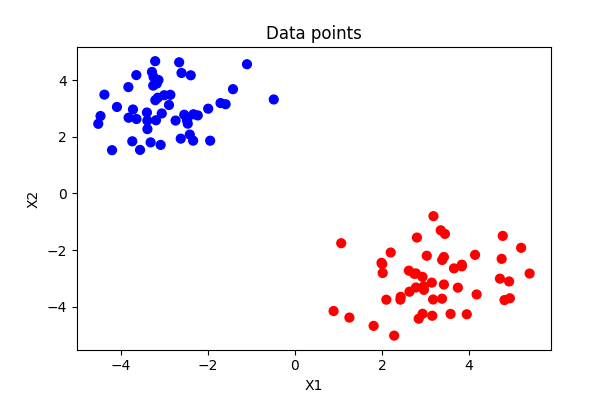
\includegraphics[width=0.5\textwidth]{1_datapoint.png}
    \caption{Data points}
    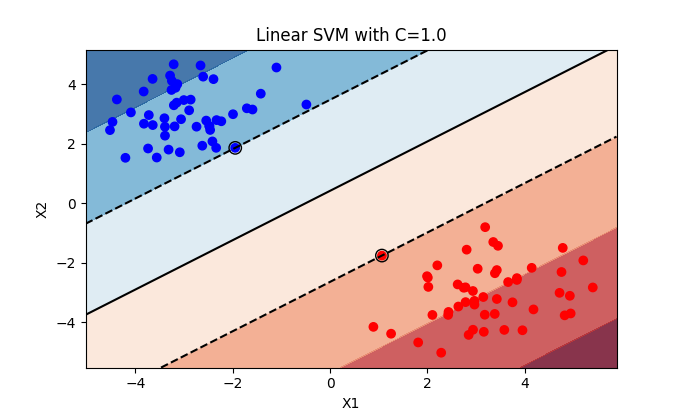
\includegraphics[width=0.5\textwidth]{1_a.png}
    \caption{Plot for a}
    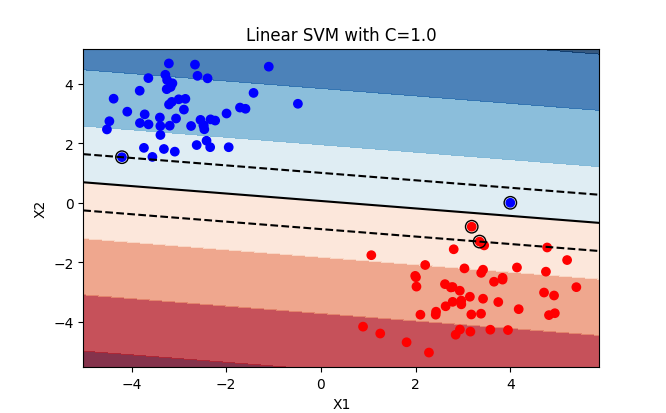
\includegraphics[width=0.5\textwidth]{1_b.png}
    \caption{Plot for b}
  \end{center}
\end{figure}

\noindent
The decision boundary changed almost horizontal to X1 when the new point because
the original decision boundary cannot classify the new point correctly.\\
When $C$ is large, it means minimizing of $\sum_{i=1}^{m}\xi_i$ is much important
than minimizing of $||w||^2$. It means the decision boundary tries to minimize
the size and the number of the margin constraint violations when $C$ is large.
Thus, the margin will be narrower, the number of support vectors and samples
that violates margin constraint will be smaller.

\clearpage

\begin{figure}[h]
  \begin{center}
    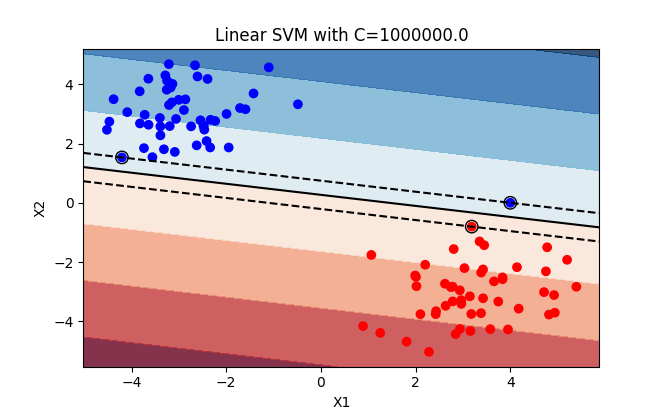
\includegraphics[width=0.5\textwidth]{1_c_6.png}
    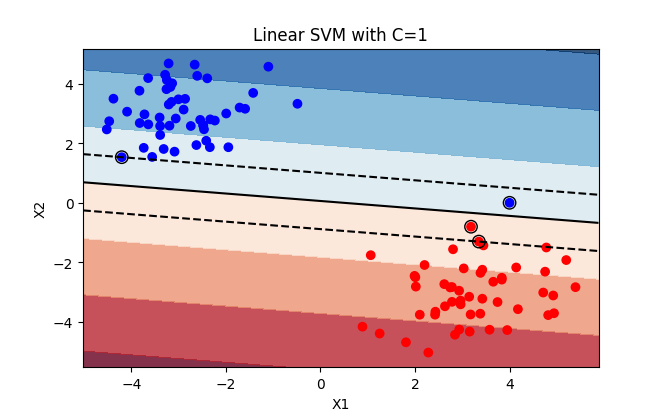
\includegraphics[width=0.5\textwidth]{1_c_0.png}
    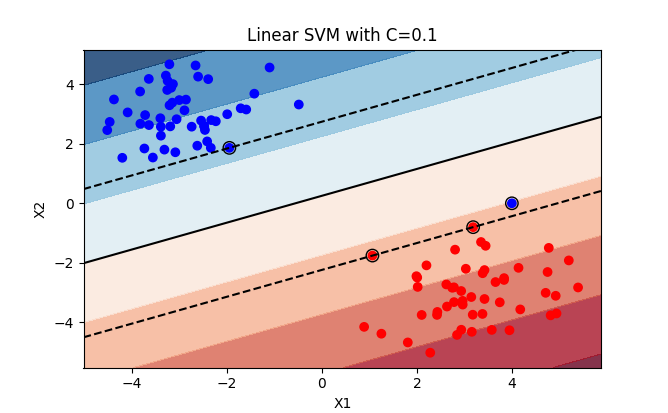
\includegraphics[width=0.5\textwidth]{1_c_-1.png}
    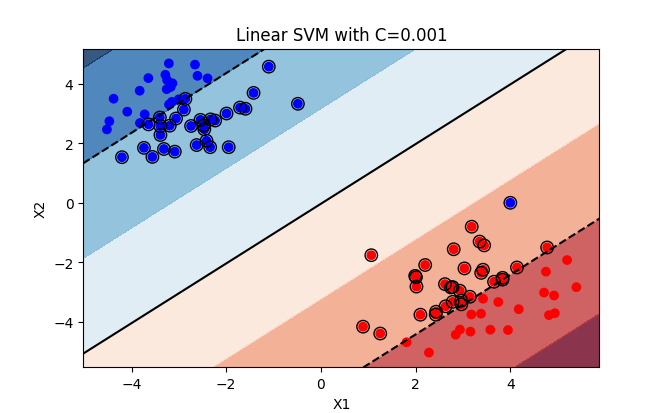
\includegraphics[width=0.5\textwidth]{1_c_-3.png}
    \caption{Plot when $C=10^6, 10^0, 10^{-1}, 10^{-3}$}
  \end{center}
\end{figure}

\clearpage

\section{Nonlinear (kernal) SVM}

\subsection*{Results}

\noindent
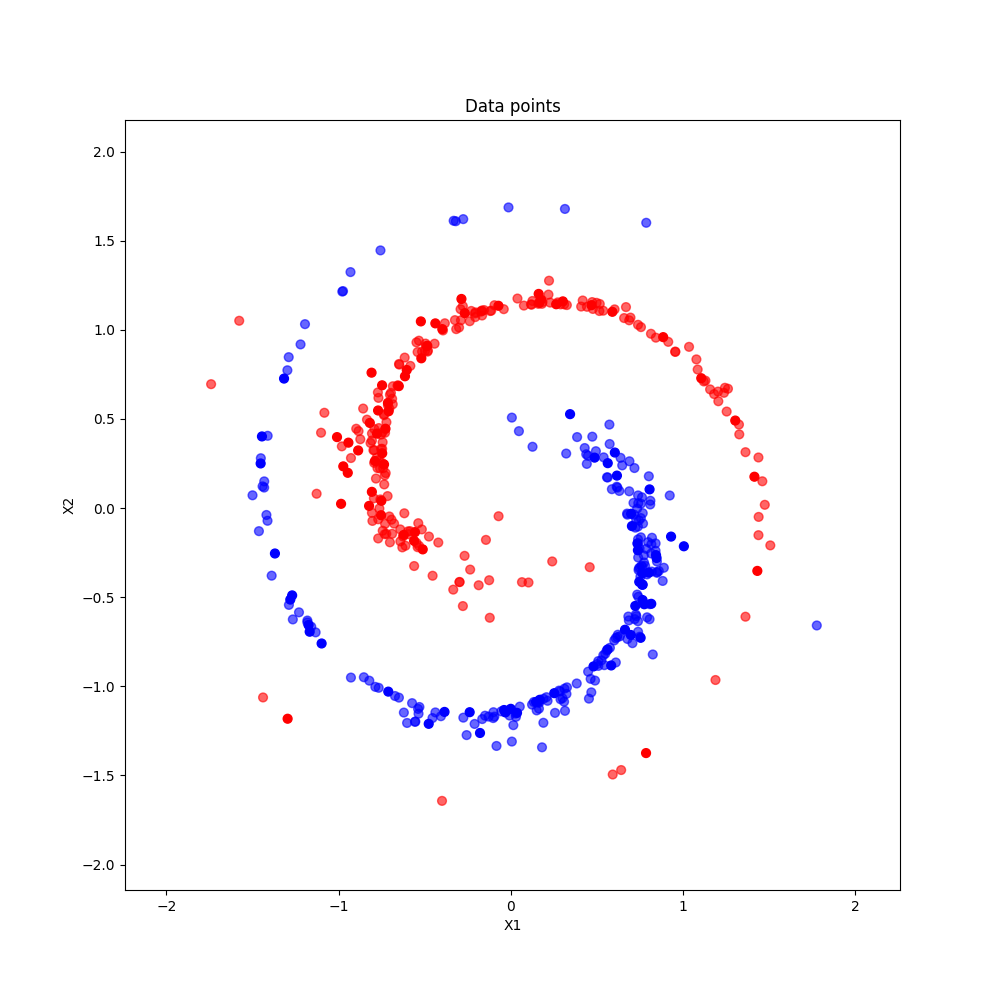
\includegraphics[width=0.5\textwidth]{nonlinear_data.png}%
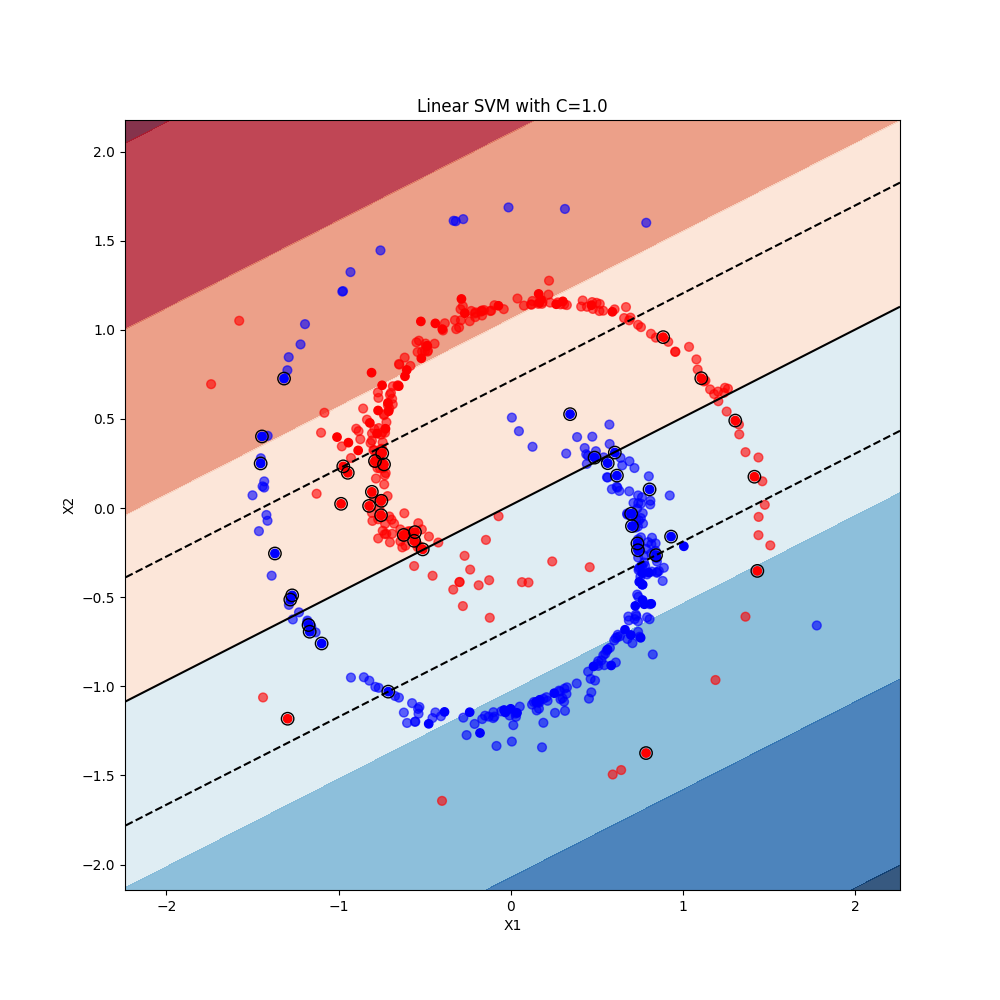
\includegraphics[width=0.5\textwidth]{linear_fit.png}\\[2em]
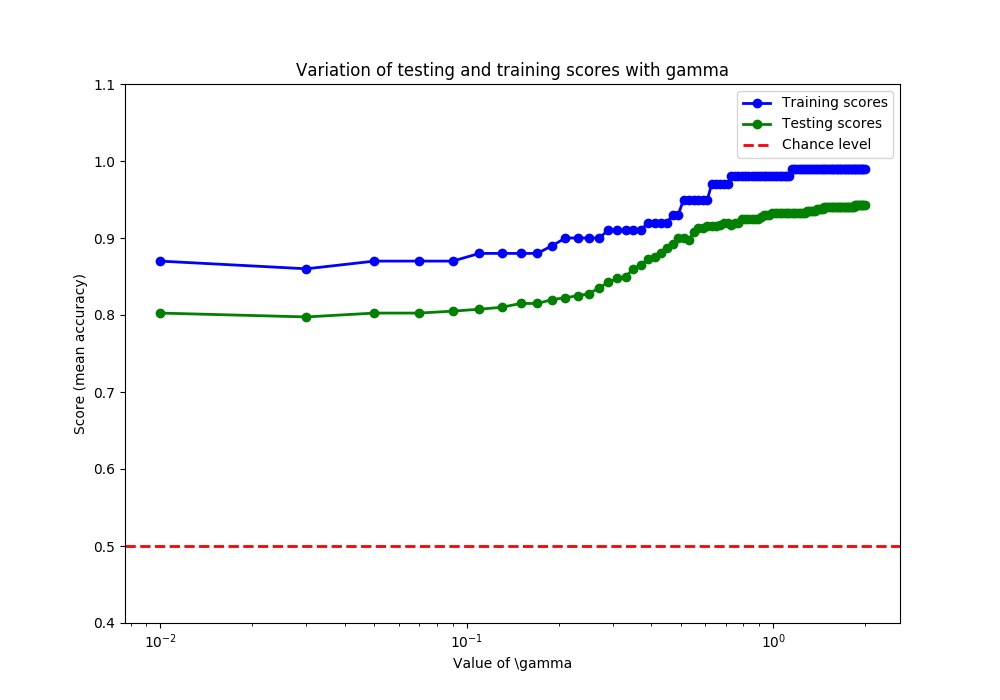
\includegraphics[width=0.5\textwidth]{rbf_error.png}%
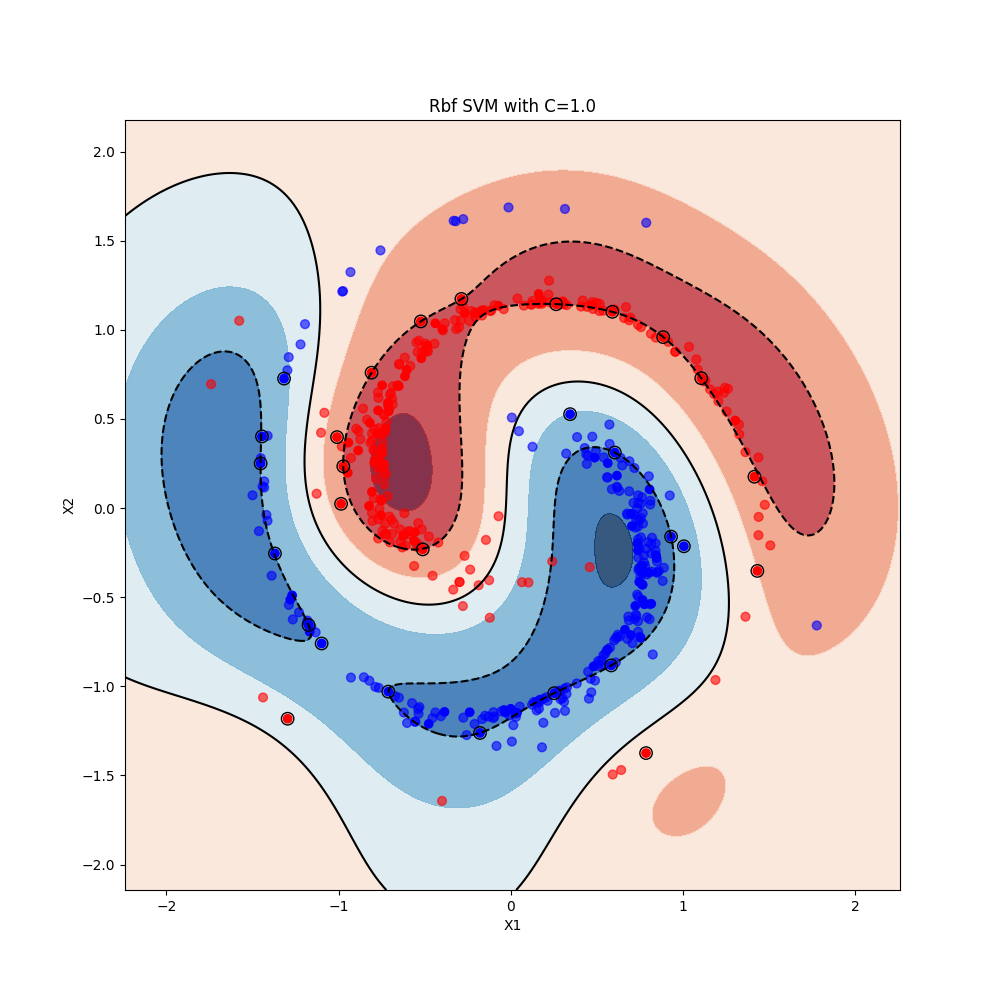
\includegraphics[width=0.5\textwidth]{rbf_fit.png}\\[2em]
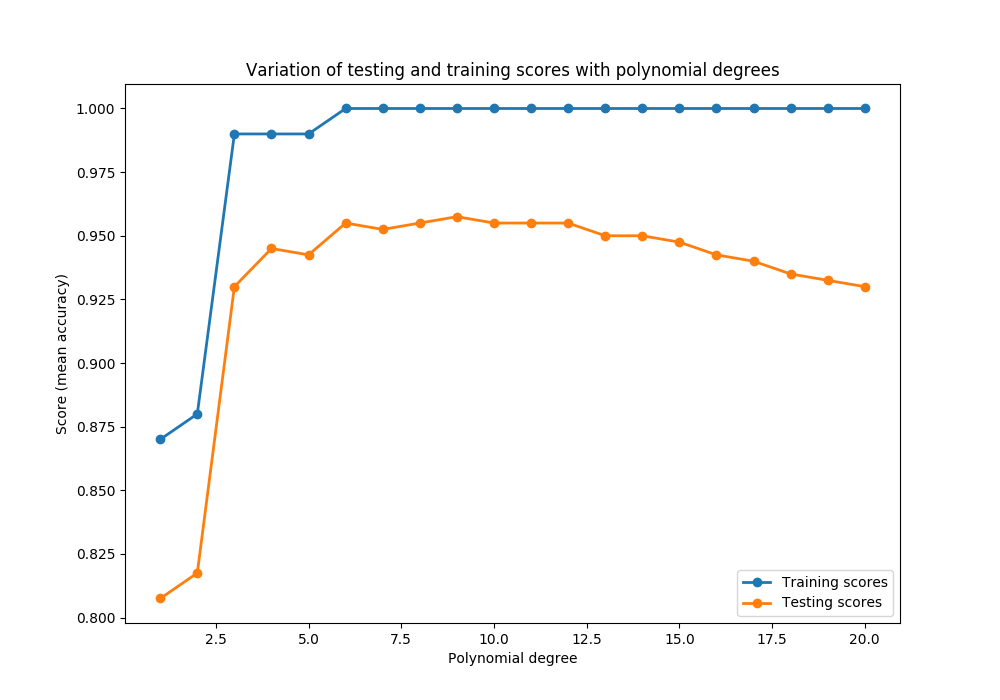
\includegraphics[width=0.5\textwidth]{poly_error.png}%
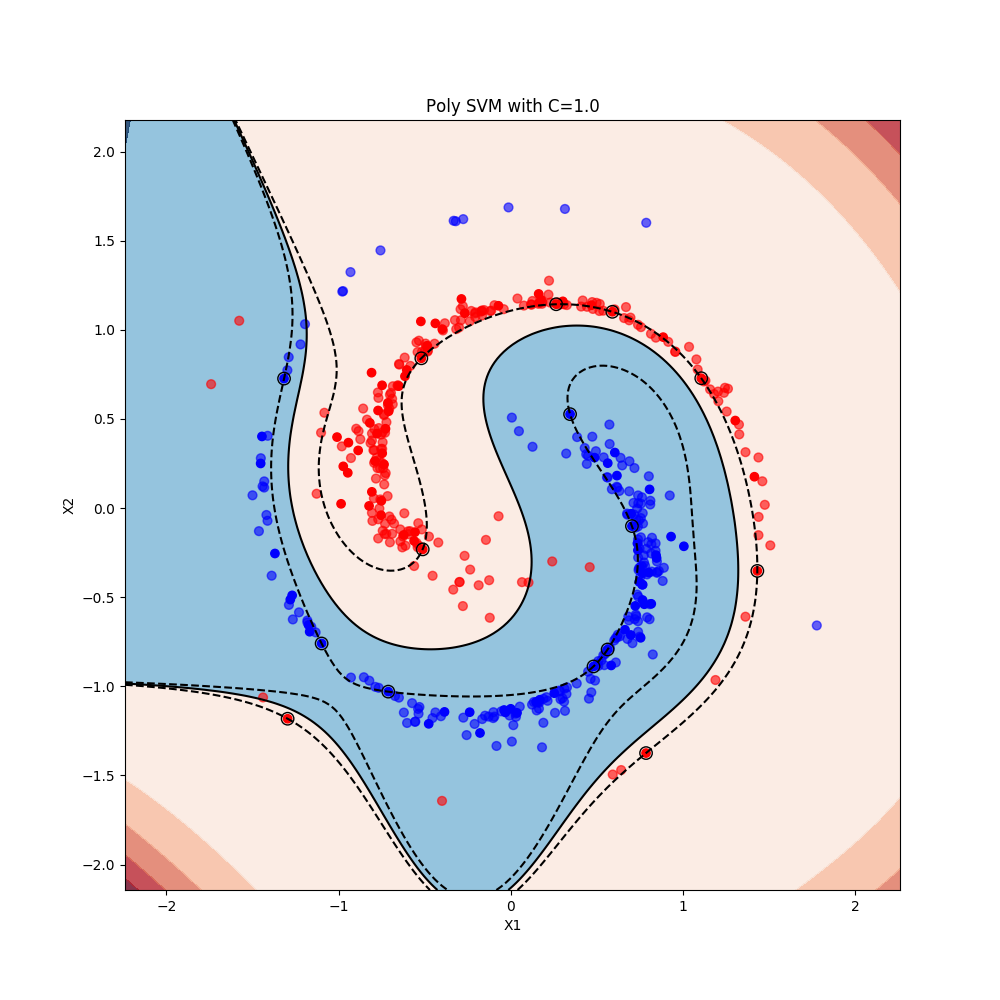
\includegraphics[width=0.5\textwidth]{poly_fit.png}\par

The above figures depict (left to right, top to bottom)

\begin{enumerate}
	\item Training data used for all algorithms
	\item A Linear SVM convergence
	\item Error in a RBF SVM plotted against the gamma value used in the kernel
	\item The most proficient RBF SVM
	\item Error in a Polynomial SVM plotted against the polynomial degree used in the kernel
	\item The most proficient Polynomial SVM
\end{enumerate}


\subsection*{Discussion}

Our Polynomial SVM had the best performance with a score of .9575 with degree 9.  The RBF SVM performed second best, scoring .9425 with a gamma of 1.85, and the Linear SVM exhibited the worst performance at .8125 .  Since the data is not linearly seperable, it is clear why the Linear SVM performed poorly.  The polynomial model outperformed the RBF model because it was able to more accurately model the central region $(-.5 < x_1, x_2 < .5)$.  It is worth noting that both models struggled with this region, with both having a significant number of misclassified examples in the region.

In general, it can be seen that a high number of Support Vectors correlates to complex decision boundaries, although this is obviously not the case for linear models.  Despite the testing results, I believe the RBF model produces a better generalization of the data, as it places the decision boundary more accurately between data points than other models.
\clearpage

\section{Multiclass classification}
\begin{figure}[h]
  \begin{center}
    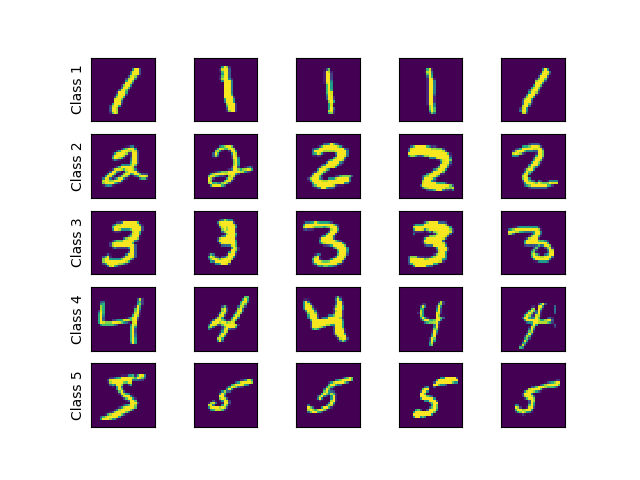
\includegraphics[width=0.5\textwidth]{3.png}
    \caption{Data samples}
  \end{center}
\end{figure}
\begin{itemize}
  \item Multiclass classification must be performed whenever data falls into more than two classes.  In this instance, we are classifying images representing digits into one of 5 classes, 1 class for each digit 1 through 5.  One such multiclass classification method is 'One-versus-All' (OVA), where each class has its own binary classifier.  Each binary classifier considers a separate class as the class with positive label, and all other data points as the class with negative label.  For new points, the class of the classifier that assigns the new point a positive value is taken as the new point's class.  For data with $N$ categories, 'One-versus-Rest' classification requires $N$ binary classifiers, one for each class. In this case, 5 classifiers are needed.
Another method is 'One-versus-One' (OVO).  With this strategy, a binary classifier is trained between for each pair of classes.  For example, if we are classifying data where all points fall into 1 of 3 classes, A, B, and C, then we would use 3 binary classifiers, for the pairs (A,B), (B,C), and (A,C).  These binary classifiers classify along the two classes that define them (A and B for the first classifier of the previous example), and ignore all other data points.  To determine the class of a point, all classifiers 'vote' on the class of the point, and the point is assigned to whichever class receives the most votes.  For $N$ categories, this approach requires $N(N-1)/2$ classifiers. In this case, 10 classifiers are needed.
\end{itemize}
\begin{figure}[h]
  \begin{center}
    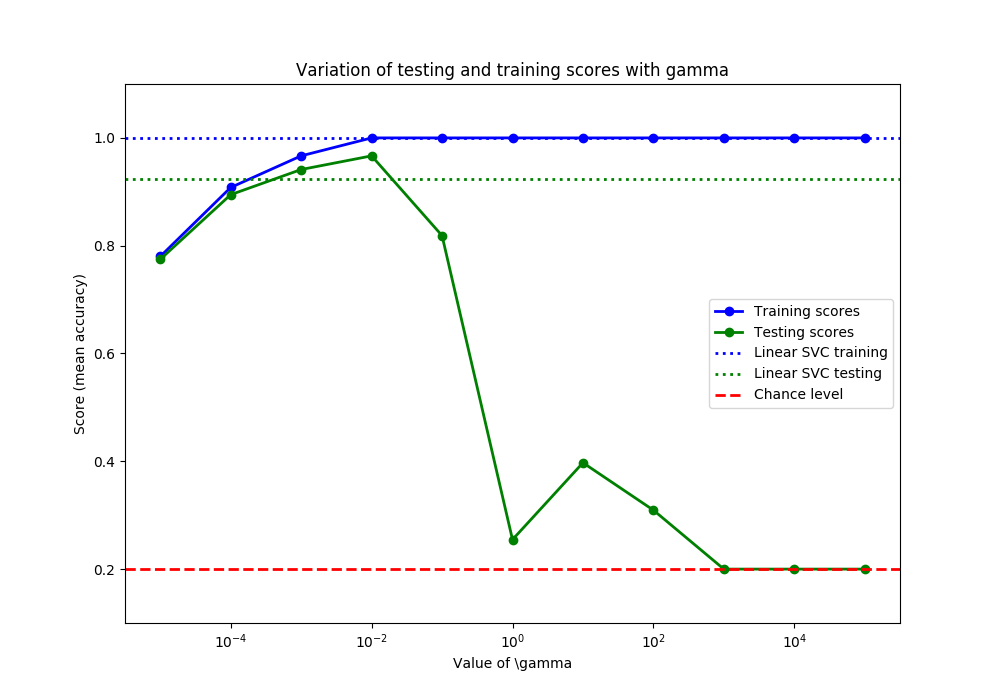
\includegraphics[width=0.7\textwidth]{3_a.png}
    \caption{Plot for a}
  \end{center}
\end{figure}
\begin{itemize}
  \item We found that the Linear kernel performed surprisingly well on this problem.  One explanation is that since we are working in a very high-dimensional space (28 by 28 images result in 784 dimensions), it is probable that a data set is largely or entirely linearly separable.
  \item Digit 5 was the most misclassified digit. 19 digits were misclassified as Digit 5 and 18 of them were digit 3 actually.
\end{itemize}
\begin{figure}[h]
  \begin{center}
    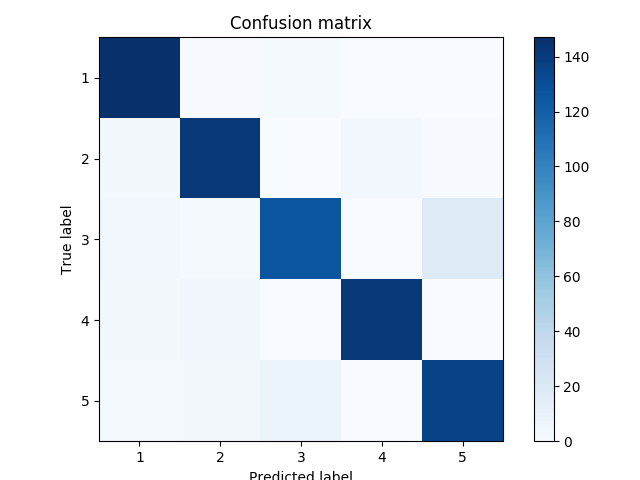
\includegraphics[width=0.5\textwidth]{3_b_cm.png}
    \caption{Confusion Matrix}
    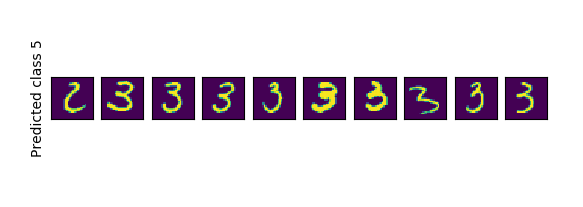
\includegraphics[width=0.7\textwidth]{3_b_err.png}
    \caption{Most misclassified digit}
  \end{center}
\end{figure}
\begin{itemize}
  \item We don't know how the classifier works exactly. However, given that 9 out
    of 10 misclassified images were digit 3, it might be hard to seperate samples
    of digit 3 and 5 linearly.
\end{itemize}
\end{document}
